% vim: set textwidth=78 autoindent:

% when the revision of a section has been finalized,
% comment out the following line:
%\updatedisclaimer

\section{Topology}\label{sec:topology}
\begin{tabular}{p{3.5cm}p{6cm}p{6cm}}
\multirow{2}{*}{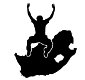
\includegraphics[width=2.5cm]{logo}} & Objectives: &
Understanding topology in vector data. \\
& & \\
& Keywords: & 
Vector, toplology, topology rules, topology errors, search radius, snaping
distance, simple feature  \\
\hline
\end{tabular}

\subsection{Overview}

\textbf{Topology} expresses the spatial relationships between connecting or
adjacent
vector features (points, polylines and polygons) in a GIS. Topological or
topology-based data are useful for detecting and correcting digitising errors
(e.g. two lines in a roads vector layer that do not meet perfectly at an
intersection). Topology is necessary for carrying out some types of spatial
analysis, such as network analysis. 
Imagine you travel to London. On a sightseeing tour you plan to visit St.
Paul's Cathedral first and in the afternoon Covent Garden Market for some
souvenirs. Looking at the Underground map of London (see Figure
\ref{fig:londontube}) you have to find connecting trains to get from Covent
Garden to St. Paul's. This requires topological information (data) about
where it is
possible to change trains. Looking at a map of the underground, the
topological relationships are illustrated by circles that show connectivity.
Changing trains at stations allows you to move from one connected part of the
network to another.

\begin{figure}[ht]
   \begin{center}
   \caption{Topology of London Underground Network.}
\label{fig:londontube}\smallskip
   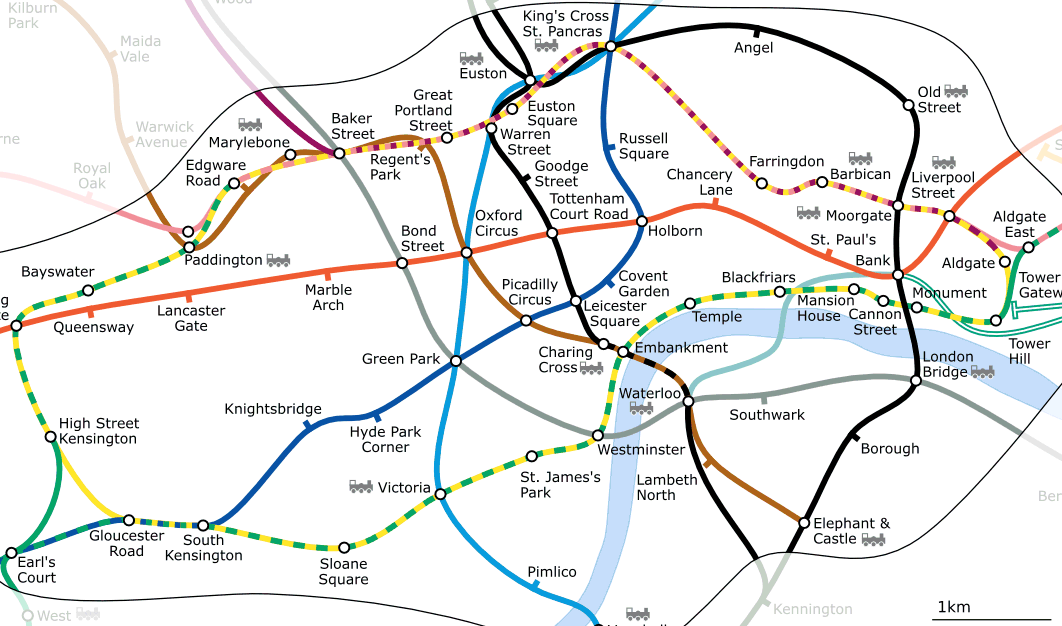
\includegraphics[clip=true, width=0.8\textwidth]{London_Underground_Zone_1_Small}
\end{center}
\end{figure}

\subsection{Topology errors}

There are different types of topological errors and they can be grouped
according to whether the vector feature types are polygons or polylines.
Topological errors with \textbf{polygon} features can include unclosed
polygons, gaps
between polygon borders or overlapping polygon borders. A common topological
error with \textbf{polyline} features is that they do not meet perfectly at a
point (node). This type of error is called an \textbf{undershoot} if a gap
exists between the lines, and an \textbf{overshoot} if a line ends beyond the
line it should connect to (see Figure \ref{fig:underovershoot}).  

\begin{figure}[ht]
   \begin{center}
   \caption{Undershoots (1) occur when digitised vector lines that should
connect to each other don't quite touch. Overshoots (2) happen if a line ends
beyond the line it should connect to. Slivers (3) occur when the vertices of
two polygons do not match up on their borders.}
\label{fig:underovershoot}\smallskip
   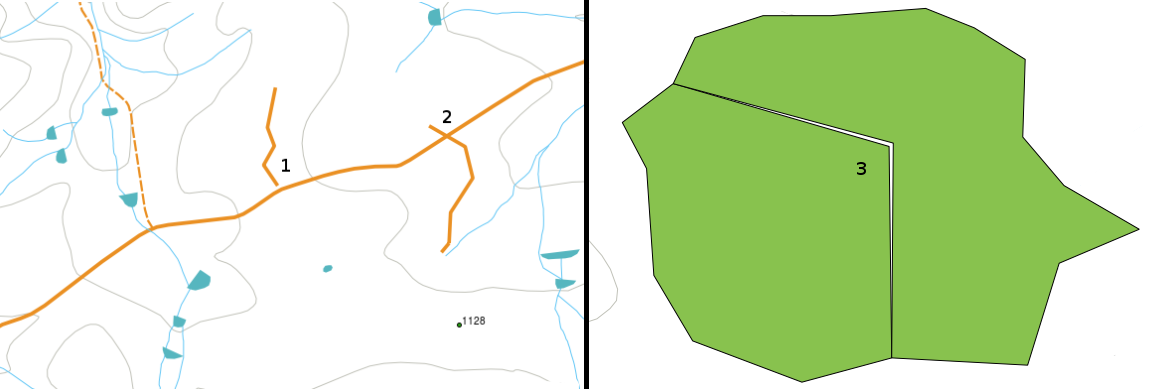
\includegraphics[clip=true, width=\textwidth]{sliver-over-undershoot}
\end{center}
\end{figure}

The result of overshoot and undershoot errors are so-called 'dangling nodes'
at the end of the lines. Dangling nodes are acceptable in special cases, for
example if they are attached to dead-end streets. 
Topological errors break the relationship between features. These errors need
to be fixed in order to be able to analyse vector data with procedures like
network analysis (e.g. finding the best route across a road network)  or
measurement (e.g. finding out the length of a river). In addition to topology
being useful for network analysis and measurement, there are other reasons
why it is important and useful to create or have vector data with correct
topology. Just imagine you digitise a municipal boundaries map for your
province and the polygons overlap or show slivers. If such errors were
present, you would be able to use the measurement tools, but the results you
get will be incorrect. You will not know the correct area for any
municipality and you will not be able to define exactly, where the borders
between the municipalities are. 
It is not only important for your own analysis to create and have
topologically correct data, but also for people who you pass data on to. They
will be expecting your data and analysis results to be correct!

\subsection{Topology rules}

Fortunately, many common errors that can occur when digitising vector
features can be prevented by topology rules that are implemented in many GIS
applications. 
Except for some special GIS data formats, topology is usually not enforced by
default. Many common GIS, like QGIS, define topology as relationship rules
and let the user choose the rules, if any, to be implemented in a vector
layer. 
The following list shows some examples of where topology rules can be defined
for real world features in a vector map.

\begin{itemize}
\item Area edges of a municipality map must not overlap.
\item Area edges of a municipality map must not have gaps (slivers).
\item Polygons showing property boundaries must be closed. Undershoots or
overshoots of the border lines are not allowed.
\item Contour lines in a vector line layer must not intersect (cross each other). 
\end{itemize}

\subsection{Topological tools}

Many GIS applications provide tools for topological editing. For example in
QGIS you can \textbf{enable topological editing} to improve editing and maintaining
common boundaries in polygon layers. A GIS such as QGIS 'detects' a shared
boundary in a polygon map so you only have to move the edge vertex of one
polygon boundary and QGIS will ensure the updating of the other polygon
boundaries as shown in Figure \ref{}(1).
 
Another topological option allows you to prevent \textbf{polygon overlaps}
during
digitising (see Figure \ref{}(2)). If you already have one polygon, it
is possible with this option to digitise a second adjacent polygon so that
both polygons overlap and QGIS then clips the second polygon to the common
boundary.

\begin{figure}[ht]
   \begin{center}
   \caption{(1)Topological editing to detect shared boundaries, when moving
vertices. When moving a vertex, all features that share that vertex are
updated. (2) To avoid polygon overlaps, when a new polygon is digitised
(shown in red) it is clipped to avoid overlapping neighbouring areas.}
\label{fig:topotools}\smallskip
   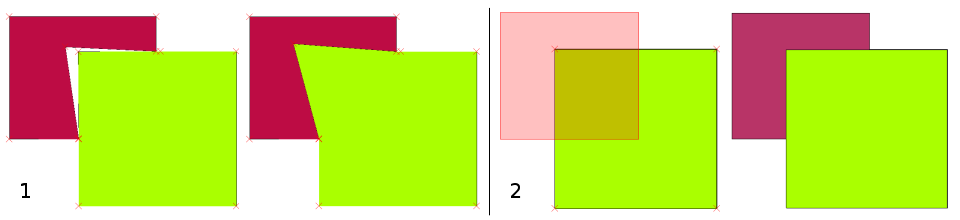
\includegraphics[clip=true, width=\textwidth]{topoediting}
\end{center}
\end{figure}

\subsection{Snapping distance}

Snapping distance is the distance a GIS uses to search for the closest vertex
and / or segment you are trying to connect when you digitise. A
\textbf{segment} is a
straight line formed between two vertices in a polygon or polyline geometry.
If you aren't within the snapping distance, a GIS such as QGIS will leave the
vertex where you release the mouse button, instead of snapping it to an
existing vertex and / or segment (see Illustration 4 below).

\begin{figure}[ht]
   \begin{center}
   \caption{The snapping distance (black circle) is defined in map units
(e.g. decimal degrees) for snapping to either vertices or segments.}
\label{fig:snapping}\smallskip
   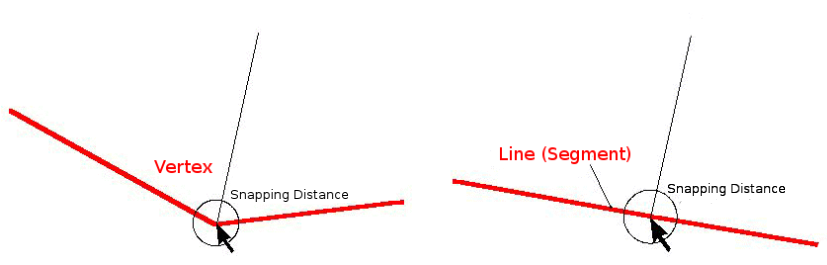
\includegraphics[clip=true, width=\textwidth]{snapping}
\end{center}
\end{figure}

\subsection{Search Radius}

Search radius is the distance a GIS uses to search for the closest vertex you
are trying to move when you click on the map. If you aren't within the search
radius, the GIS won't find and select any vertex of a feature for editing. In
principle, it is quite similar to the snapping distance functionality. 
Snapping distance and search radius are both set in map units so you may
need to experiment to get the distance value set right. If you specify a
value  that is too big, the GIS may snap to a wrong vertex, especially if you
are dealing with a large number of vertices close together. If you specify
the search radius too small the GIS application won't find any feature or
vertex to move or edit.

\subsection{Common problems / things to be aware of}

Topology is a complex representation of vector data. True topological vector
datasets are stored in special file formats that record all the relationships
between features. Most commonly used vector data formats use something called
'Simple Features' which also consists of point, line and polygon features.
Simple feature datasets are mainly designed for simplicity and for fast
rendering but not for data analysis that require topology (such as finding
routes across a network). Many GIS applications are able to show topological
and simple feature data together and some can also create, edit and analyse
both.

\subsection{What have we learned?}

Let's wrap up what we covered in this worksheet:

\begin{itemize}
\item \textbf{Topology} shows the spatial relation of neighbouring vector features.
\item Topology in GIS is provided by \textbf{topological tools}. 
\item Topology can be used to \textbf{detect and correct digitizing errors}.
\item For some tools, such as \textbf{network analysis}, topological data is
essential.
\item \textbf{Snapping distance} and \textbf{search radius} help us to
digitise topologically correct vector data.
\item \textbf{Simple feature} data is not a true topological data format but
it is commonly used by GIS applications.
\end{itemize}

\subsection{Now you try!}

Here are some ideas for you to try with your learners:

\begin{itemize}
\item Mark your local bus stops on a toposheet map and then task your learners to
find the shortest route between two stops.
\item Think of how you would create vector features in a GIS to represent a
topological road network of your town. What topological rules are important
and what tools can your learners use in QGIS to make sure that the new road
layer is topologically correct?  
\end{itemize}

\subsection{Something to think about}

If you don't have a computer available, you can use a map of a bus or railway
network and discuss the spatial relationships and topology with your
learners.

\subsection{Further reading}

\textbf{Books}:

\begin{itemize}
\item Chang, Kang-Tsung (2006): Introduction to Geographic Information Systems. 3rd
Edition.  McGraw Hill. (ISBN 0070658986)
\item DeMers, Michael N. (2005): Fundamentals of Geographic Information Systems.
3rd Edition. Wiley. (ISBN 9814126195)
\end{itemize}

\textbf{Websites}:
 
\url{http://www.innovativegis.com/basis/primer/concepts.html} \\
\url{http://en.wikipedia.org/wiki/Geospatial\_topology}

The QGIS User Guide also has more detailed information on topological editing
provided in QGIS.

\subsection{What's next?}

In the section that follows we will take a closer look at \textbf{Coordinate
Reference Systems} to understand how we relate data from our spherical earth
onto flat maps!





